\documentclass[11pt,twoside,a4paper]{article}
\usepackage{fancyhdr}
\usepackage[UTF8]{ctex}
\usepackage[centering]{geometry}
\usepackage{graphicx}
\usepackage{setspace}
%\usepackage{listings}
%\usepackage[colorlinks=true,linkcolor=blue,urlcolor=blue,citecolor=black]{hyperref}
%
%\usepackage{algorithm}  
%\usepackage{algorithmicx}  
%\usepackage{algpseudocode}  
%\usepackage{amsmath}  
%\usepackage{graphicx}
\begin{document}
	\begin{figure}[h]
		\centering
		% Requires \usepackage{graphicx}
		
\includegraphics[width=0.8\textwidth]{graph/logo.png}\\
	\end{figure}
\thispagestyle{empty}
\begin{center}
	\doublespacing
	\huge 当代中国医疗的深度思考
	
	\Large 1160300329\ 黄海 
	
	\Large 1160300308\ 干寅雷
	
	\Large 1160300311\ 汤嘉琦
	
	\Large 1160300312\ 靳贺霖
	
	\Large 1160300314\ 朱明彦
\end{center}
	\singlespacing
%	\title{当代中国医疗的深度思考}
%	
%	\author{1160300329\ 黄海\\1160300308\ 干寅雷\\1160300311\ 汤嘉琦\\
%		1160300312\ 靳贺霖\\1160300314\ 朱明彦\\1603003班}
%	\author{Paolo Ienne\\ 
%		Swiss Federal Institute of Technology\\ Microcomputing Laboratory \\ IN-F 
%		Ecublens, 1015 Lausanne, Switzerland\\ Paolo.Ienne@di.epfl.ch\\ 
%		% For a paper whose authors are all at the same institution, 
%		% omit the following lines up until the closing ``}''. 
%		% Additional authors and addresses can be added with ``\and'', 
%		% just like the second author. 
%		\and 
%		Second Author\\ 
%		Institution2\\ 
%		First line of institution2 address\\ Second line of institution2 address\\ 
%		SecondAuthor@institution2.com\\ 
%	} 
	\newpage
	\pagestyle{fancy}
	\thispagestyle{fancy}
	\lhead{当代中国医疗的深度思考}
	\chead{}
	\rhead{Harbin Institute of Technology}
	\lfoot{}
	\cfoot{}
	\rfoot{\thepage}
%	\maketitle
	
	\newpage
	\begin{center}
	\textbf{Abstract}	
	\end{center}
		对于当前的中国医疗,不可否认其中存在问题。在下面的讨论中,我们将对于中国医疗的价格高低,通过对比的方式利用辩证法的原理,进行分析。合理看待中国医疗价格中存在的问题,并探寻问题产生背后的原因。
	\begin{flushleft}
	\textbf{Keyword:中国,\ 医疗问题,\ 医患关系,\ 医疗资源,\ 医疗成本,\ 医疗保险,\ 医疗改革}
	\end{flushleft}

	\newpage
	
	\tableofcontents
	
	\newpage
	
	\section{中国医疗成本}
		\subsection{简述}
		对于中国医疗成本的高低,如果我们仅仅针对中国的情况纵向来看,有失其完整性。基于此,我们使用辩证法的思想,通过对比的方式,将中国与发展中国家代表(印度)以及发达国家代表(美国)进行横向的比较。通过这种方式,进而来说明中国医疗成本在世界中的地位和存在的问题。对于医疗问题中的不同方面,如医务人员薪酬方面,医疗器械方面和药品价格三个方面,使用上面的思路进行分析。
		\subsection{医务人员方面}
		对于中国的医务人员,先说结论:\textbf{在世界的各个国家之中,属于低收入的医务人员群体}。
		
		在这里,我们选取了一个来自中国985院校的医学硕士毕业生(下面简称为“985学生”)作为对比的对象,与中国城镇居民人均收入进行对比。可以发现,985学生的平均收入为$80000$元每年,与其对比的中国的城镇居民的人均收入已经达到了$30000$元每年。
		
		对于个例我们只是作为一种说明,下面借用2016年丁香园医生对于中国医务人员薪酬的调查\cite{ref1}来看,中国的医务人员的平均年薪为$85000$元,对比2016年度全国城镇居民人均可支配收入$33616$元\cite{ref2}来看,已经是其3倍左右,我们可以说医务人员的收入不低,进而我们可以说医疗成本至少不低,因为治病的医生的工资成本很高。但是由于没有很好的中位数数据,可能有不少被平均的情况,我们只能得到以上的结论。
		\begin{figure}[htb]
			\centering
			% Requires \usepackage{graphicx}
			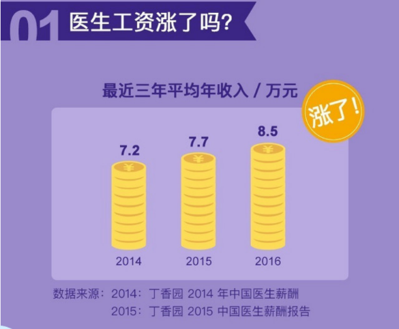
\includegraphics{graph/DingXiangyuan.png}\\
			\caption{丁香园2016年中国医务人员薪酬调查}
		\end{figure}
	
		我们可以看到美国的医生平均收入已经达到了$28$万美元以上\cite{ref3},相比美国人均年收入$42372$美元,已经超出6倍有余,这是中国医生所远远不能与之相比的。
		
		
		再来看印度,由于数据的问题我们不能找到具体的印度医生收入的直接证明,但是相信看过生活大爆炸的同学都会对Raj的父亲的收入有着极深的印象。根据较少数据规模的统计我们可以知道,在印度医生的工资分布比较分散,在印度,一个家庭医生的收入约为16万到126万卢比不等,并且由于印度允许医生在医院之外行医所以工资更加难以计算。我们可以参考的另一个数据是在印度医学院毕业的本科生的薪资一般为1000美元一个月,对比印度的人均年收入1500美元左右,也称得上是高收入人群了。
		
		\begin{figure}[htb]
			\centering
			% Requires \usepackage{graphicx}
			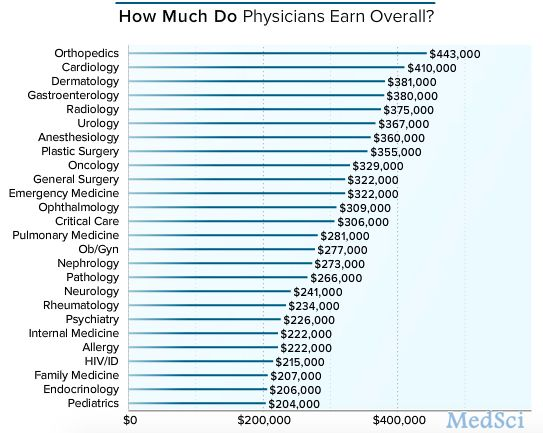
\includegraphics[width=0.8\textwidth]{graph/20160402203312581.png}\\
			\caption{2016年Medscape医生收入调查}
		\end{figure}
		
		另外中国医生除了薪资不高还有这些问题,工作强度大,收入满意度低还有升职加薪困难。这些低收入高压力之间的矛盾让很多医生都不堪重负。
		
		可以说无论是印度还是美国,医生的社会地位和薪资状况在其社会环境中都出于中上地位相比,中国的医生真的可以说是“价廉”了,换句话说医生的薪资很低,中国的医疗成本应该不高。
		
		\subsection{医疗器械方面}
		这个方面我们结合着来看,以心血管支架为例,某种血管支架在我国现行价格为$1.8$万元左右人民币,而产地美国却是$8000$元人民币。中间超过一倍有余的价格都是来自于经销商的层层剥皮。这仅仅是一个方面,同样跟血管支架有着类似情况的医疗器械,小到一个几百美元的血管钳,上到单机价格$2000$万人民币的达芬奇手术机器人,中国无不使用远高于国外价格的来进口,而不能用国产设备代替。
		
		也就是中国无法打破国外的技术壁垒,只能用远低于发达国家国民收入的百姓的辛苦钱去承担与发达国家百姓相同甚至更高的医疗器械费用。
		
		\subsection{药品方面}
		中国是有着几十年不涨价的药物,但是近些年来不断出现的出国去买靶向药的情况屡有发生,这与中国国产没有靶向药不无关系。做一个直接的价格对比“特罗凯(抗癌药)在2016年8月份宣布降价,但仍要$4000$多元一盒。
		
		又如,和特罗凯同属抗癌靶向药的格列卫,国内正版的价格仍要$2$万多元一盒,仿制药物$3000$多元,而印度版格列卫一盒只需$200$多元。”
		
		虽然现在有了医疗报销的体系,在部分发达的地区报销格列卫的比例超过$90\%$,但仍有$2000$多元一盒的高昂价格。这相差十几倍的价格仍然需要中国患者来承担,这些对比我们可以坚定地说中国的医疗成本很高。
		
		\subsection{简要分析}
		结合三个方面辩证来看,我们不能直接说中国的医疗成本很高,因为中国医生收入真的不高;也不能说中国的医疗成本低,因为无论药品或是器械,国内的价格远高于国外。
		
		那么我们只好用事实进行佐证,在现在,即使有着大病保险和医疗保险的极高覆盖,但对于很多的中国居民“一病回到解放前”真的是一种普遍情况,所以我们可以认为中国的医疗成本确实很高,这种高不是来自于平时的头疼脑热所用掉的那些医保以内的药物,而是当真正有着严重疾病发生的时候那种高昂的医疗成本造成的。
		
		\section{农村和城市医疗现状对比}
		\subsection{农村医疗的问题}
		\paragraph{投入不足}
		乡村医疗卫生事业投入不足,这是一个带有共性的问题。党的十八大以来,政府虽然对乡村特别是贫困乡村卫生事业的投入有所增长,但投入标准仍旧偏低。多数乡村医疗卫生服务机构的医疗技术人员学历较低,很多都是中专毕业,医务人员水平有限,队伍结构老化严重。不少医疗机构大都安于现状,提升发展动力不足,没有主动扩充人员、优化队伍和积极性。这造成了一些乡村医疗卫生机构人才匮乏、医术不精、服务质量不高等问题。
		
		\paragraph{基础薄弱}
		各级政府虽然对乡村医疗机构的基础设施及医疗设备投入了资金,但仍不能满足患者的医疗需求,特别是在一些边远的贫困山区更是如此。由于基础投入不足,病房陈旧、紧缺等问题较为突出。基本建设较薄弱,医疗设备陈旧,医疗水平得不到提高,不能满足患者要求。同时,乡村医疗卫生服务机构还普遍存在着药品种类少且不齐全、短缺等现象。
		\paragraph{人才缺乏}
		人才结构不够合理,层次较低,不利于乡村医疗卫生事业的可持续发展。由于现有的人事与分配制度较为僵化,医务人员收入不高,乡村医疗卫生院室基础条件较为落后,无法为高端人才创造较好的事业环境,一些毕业于知名院校的医生不愿到乡村医疗院室来,还有少数医疗人才因工资太低而离开等。
		资源不均。乡村居民“看病难、看病贵”的原因是多方面的。一方面,乡村患者小病拖、大病扛,病人支付能力有限不愿意到医院看病,结果是小病拖成大病进而拖成危重病。另一方面,基层医院资源匮乏,就医条件有限,患者涌向省、市、区级医疗条件好、设备先进的医院,最终又演变成新的“看病难,看病贵”现象。
		\paragraph{管理落后}
		因条件限制,乡村医疗卫生院室无法留住专业的高素质人才,这自然也包括管理方面的人才,所以导致乡村医疗卫生院室严重缺乏先进的管理经验,不仅院室岗位存在设置不合理的情况,同时,在扩建地管理上也存在许多纰漏,比如,有的乡镇医院不结合自身实际情况进行扩建,盲目追求发展,然而在扩建后又没有得到有效利用,这就造成了资源的浪费,而有相当的村又仅有一间简陋的卫生室,有的贫困村甚至就没有。
		
		\subsection{农村和城市医疗条件对比}
		城市和农村卫生服务需求率均较高, 除急、慢性病防治、普及健康知识城市和农村需求率无差别外, 其他项目均城市高于农村。社区提供给城市和农村家庭的医疗服务以常见病治疗为主, 多数预防服务项目供给率城市高于农村。 除儿童计划免疫外, 在优生优育、妇幼保健、传染病防治、健康体检、普及健康知识、康复医疗、建立健康档案等方面总需求均大于总供给。 对社区卫生服务质量要求城市家庭高于农村, 希望社区提供全天候卫生服务形式;绝大多数家庭能承担各项医疗费用, 因病致贫基本没有。从住宅到医院的距离农村大于城市, 特别是农村家庭到县医院路途费时较多。
		
		\subsection{农村和城市医保现状}
		\paragraph{城镇职工基本医疗保险:}
		以个人缴费为主、财政补助为辅,可以享受到基本医疗保险和个人负担补助。
		\paragraph{城镇居民基本医疗保险:}
		工资扣除,参保者可以享受到基本医疗保险、公务员医疗补助保险、大额医疗费用补助。
		\paragraph{新型农村合作医疗:}
		缴费水平较低,保障水平较低,补偿疾病医疗费用,门诊等小病不在保障范围内。
		\paragraph{大病医保:}
		人人可参加,大病保险所需要的资金从城镇居民医保基金、新农合中划出。
		
		\textbf{相比较而言,农村医保体制不够完善,保障不够全面1、报销比例低;2、可适用范围受限;3、新农合在看大病方面无保障。而城市医保已经有了比较健全的体制。}
		
		\subsection{当前解决措施}
		\paragraph{城乡医疗并轨:}2017年将会在试点地区开始实行新农合和城镇居民医保并轨的方案,这也就是说,城乡医疗并轨后,农村居民可以享受到城镇居民同等的医保待遇。
		\paragraph{加大农村卫生投入力度:}扶持农村医疗卫生基础设施建设 国家财政对卫生事业的投入应适当向农村倾斜,加大对农村卫生事业的支持力度。
		\paragraph{推进农村基本药物制度改革:}把药价降下来 政府要结合实际,从制度方面入手,扎实推进农村医疗体制改革和基本药物制度改革,提高农村合作医疗报销比例,报销费用提上去,让农民能够看得起病
		\paragraph{强化卫生立法:}由于医疗卫生改革领域的复杂性,必须通过立法来确保多层次医疗保障体系和农村医疗卫生事业的改革与建设。
		
		\section{医患关系}
		\subsection{医患关系严峻的背景}
		\begin{itemize}
		\item 2000年8月,武汉市第六医院,医务科一名人员遭患者硫酸毁容
		\item 2003年9月4日,四川成都市第二医院,怀孕护士惨遭干部病房患者家属殴打致流产,其丈夫也被殴打可能致残,千人签名要求严惩凶手。 
		\item 2012年3月23日,哈尔滨医科大学附属第一医院免疫科医生办公室里,一名男子突然冲入行凶,当场造成医务人员1死3伤。不久前,一张护士扇婴儿耳光的动态图片又将社会的焦点集中到了医患关系上。 
		\item 2016年11月22日上午10时许,山西长治医学院附属和平医院院内发生一起暴力伤医案件。感染性疾病科1名医生在院内会诊途中,突然遭到1名男子持刀袭击,被害人身遭9处刀伤,其中1处刺破心脏,导致心脏破裂,心包填塞。
		\end{itemize}
		
		\subsection{医患关系紧张的原因}
		\begin{itemize}
			\item 经济投入不足:我国现行的医疗保障体系及相关的法律、法规没有及时跟上市场经济的步伐。政府对医院的投入严重不足,医院自负盈亏的体制,都促使患者承担了过多的诊疗费用。同时,社会贫富分化,矛盾加剧的问题在费用高昂的诊疗过程中被激化。 
			\item 缺少沟通 :医患沟通不够、医疗纠纷增加,是医患关系不和谐的重要因素。基层医疗资源不足,水平欠缺,经常发生误诊的现象,使得病人为寻求可靠的诊疗向大城市的三甲医院集中。医生超负荷的工作使其无力完善与患者的沟通。同时,医疗教育的制度并未在医患沟通技能中给予学生强化训练,使得医生缺乏良好的沟通技能。 
			\item 缺少信任 :医患之间缺乏信任,是造成医患矛盾的一个重要原因。新闻媒体不够详实的报道,促使医患之间缺乏信任、理解,不能换位思考。部分医务人员没有设身处地替患者着想,而是较多地考虑医疗机构和自身的利益。而有些患者对医务人员也缺乏理解,不了解医学的复杂性。 
			
		\end{itemize}
		
		\subsection{缓解医患关系的方法 }
		\paragraph{医务人员转变观念是处好医患关系的基础}
		转变“医者至上”的服务观念,将患者作为一个完整的社会人来看待,用过硬的技术来减轻患者身体的病痛,用真诚的服务减缓患者沮丧无助的心理,用尊重的态度让患者感觉和医务人员处在同等地位,用人性化的关心为患者营造一个良好的就医环境。时刻不忘对患者说一句“我的治疗需要您的配合”,使医务人员和患者站在同一战线上面对共同的问题。这一点在糖尿病患者、高血压及尿毒症等患者身上体现的尤为深刻。 
		\paragraph{让患方转变观念是处好医患关系的重要条件} 
		患方是来自不同文化层次的人群,让患方转变观念需要医务人员的不断渗透。医院是实施有偿医疗行为的机构,而非福利院。医疗技术的提高需要新技术的开展和新设备的使用,而这些势必会增加患者的日均费用或者总的费用。医学是一个不断发展完善的学科,医务人员知识的更新及患者个体的差异,使得即使是专家也不敢保证自己能医好所有病人的疾病。让患者理解医务人员所实施的行为完全是为了解除患者的病痛。 
		
		\paragraph{加强医患沟通是密切医患关系的重要策略 }
		医患沟通是医患之间构筑的一座双向交流的桥梁。在医疗服务过程中,医患之间心理距离近,感情融洽,医患关系就好。在良好的医患关系中,尽管医疗机构在服务上有些缺陷,患方也能在友好的情感中予以谅解。尊重患者的知情同意权是处理医患关系的关键环节。患者的知情同意权是患者的基本权利之一。医务人员在履行某些治疗行为前,应先同患者进行交谈,包括病情,治疗的依据,治疗的原理,治疗中可能出现的问题等等均应告知患者,让患者根据自己选择是否做治疗和检查,以取得患者的主动配合,真正做到尊重患者,让患者充分享受就医的知情权和选择权。 
		
		\paragraph{提高医疗技术是密切医患关系的重要前提}
		 
		医疗技术是产生医患关系的重要前提。医务人员首先要在自己的专业领域内具备丰富的医学理论知识,让患者取得疾病的控制好转和相应的健康指导,这是取得患者信任的第一要素,对所接诊病人的相关疾病无论是否有很丰富的临床经验,都应将此疾病的病理生理、诊断、治疗等各方面的知识掌握好,在此基础上多与病人交流,告知有关疾病的治疗、保健等方面的知识。即使自己的知识一时不能满足患者的需求,也应该积极请教自己的上级医师,查阅相关资料甚至医学网站,尽自己所能为患者提供较高的技术服务。 
		\paragraph{良好的职业道德是处好医患关系的根本 }
		要有良好的医德,医德的最充分的体现是高度的责任心、同情心,应以换位思考顾及患者的需要,比如尽量减少病痛、缩短治疗时间、达到最好疗效。医生的治疗不仅是医治的结果,还包括对患者精神上的慰藉。严格按章办事,规范操作,对患者一视同仁,实际工作中灵活运用语言、行为、心理技巧沟通交流,与患方成为朋友。在诊断、治疗过程中认真细致、严谨周密、实事求是、坚决杜绝一切由于缺乏责任感而造成的拖延、差错、事故,取得患者的信任与尊重。 
		\paragraph{改善基础服务设施也会促进医患关系和谐 }
		重视医院的基础服务建设,提高病人的满意度。医院是病人接受治疗的场所,在这期间,医院就是他们暂时生活的居住地。舒适的环境是提高病人满意度的重要因素,也是改善医患关系不可忽视的因素之一。另外,医院开展“微笑服务”,提高全院医务人员的工作热情,这也是改善医患关系的重要途径,它足以弥补医院在某些方面的欠缺,让病人感觉医护人员就仿佛是他们身边的亲人,努力为自己的健康所奔波劳累。 
		\subsection{改善医患关系的意义}
		构建社会主义和谐社会,是我们党以马克思列宁主义、毛泽东思想、邓小平理论和“三个代表”重要思想为指导,全面贯彻落实科学发展观,从中国特色社会主义事业总体布局和全面建设小康社会全局出发提出的重大战略任务,反映了建设富强民主文明和谐的社会主义现代化国家的内在要求,体现了全党全国各族人民的共同愿望。我们党关于构建社会主义和谐社会的思想,开辟了社会主义社会建设理论的新境界,丰富和发展了中国特色社会主义理论。
		\begin{enumerate}
			\item 提出构建社会主义和谐社会,是对人类社会发展规律认识的深化,是对马克思主义关于社会主义社会建设理论的丰富和发展。实现社会和谐,建设美好社会,始终是人类孜孜以求的社会理想。
			\item 提出构建社会主义和谐社会,是对社会主义建设规律认识的深化,丰富和发展了中国特色社会主义理论。促进社会和谐,是社会主义的本质要求。
			\item 提出构建社会主义和谐社会,是对共产党执政规律认识的深化,是我们党执政理念的升华。构建社会主义和谐社会,进一步体现了我们党执政的本质要求。 
			\item 构建社会主义和谐社会,关系最广大人民的根本利益,关系巩固党执政的基础、实现党执政的任务,关系国家的长治久安。
		\end{enumerate}
		\subsection{构建和谐医患关系的重要意义}
		\begin{enumerate}
			\item 有利于维护良好的社会秩序和促进社会的稳定运行医患关系的状况如何,是人们社会关心状况如何的一个缩影。
			\item 有利于最大程度的实现社会的公平正义社会的公平正义,是指社会各方面的利益关系得到妥善协调,人民内部矛盾和其他社会矛盾得到正确处理。医患矛盾的解决,需要根据公平正义的原则,正确界定医方和患方的权利及义务,最大程度的实现社会的公平正义。
			\item 有利于有效地提高人民的生活质量医学的发展离不开医务人员对疾病的发生、发展及转变进行研究,而疾病不是独立于人体而存在的。构建和谐的医患关系,有利于调动医务人员的积极性和创造性,充分发挥医务人员的主观能动性,促进我国医学事业的发展,大力保障人民的健康,从而有效地提高人民的生活质量。
		\end{enumerate}
		
		\section{中国医改的历程}
		回顾中国医改的历程,我们发现,卫生事业改革发展的过程,就是保障人民健康水平这个根本目标、不断在改革发展中解决新矛盾新问题的过程。
	
		1980年,取消单位医务室,农村合作医疗解体。国务院发文允许个体医生开业行医,民营医疗市场开始兴起,医疗卫生机构开始走向社会化,企业化。1989年,国务院出台意见,强化医疗卫生市场化,实行医院分级管理体制,各级医疗单位内部独立核算、自负盈亏。由于缺乏认证和监管,各地医疗卫生技术水平,收入差距进一步加大。一些医院为了追求利益,开始出现医疗乱象。1998年,中国社会医疗保障体系建设开始。医保改革主要是城市经济体制改革的配套,并稳定剧变中的职工队伍。在很大范围内,将公费医疗制度转为医疗保险制度,由政府全包转向政府主导与市场机制结合。2009年,新一轮医改方案正式出台,提出建立健全医疗保障体系,基本公共卫生服务的均等化,实现‘重治疗“向”重预防“转变的前提。
		
		上述过程可以归结为三个阶段。第一阶段是从1978年至1996年,这一阶段是我国卫生事业解放思想、积极探索的阶段。上世纪70年代末,由于十年动乱的影响,我国医疗卫生资源严重短缺;综合国力和财力较弱,政府发展卫生事业的能力受到极大限制;同时由于平均主义和“大锅饭”盛行,医疗卫生领域服务质量受到诟病。针对医疗服务供不应求的主要矛盾,这一阶段卫生改革发展的重点是大力提高卫生服务能力,增强医疗卫生机构活力,扩大服务供给,缓解供需矛盾。同时要打破“平均主义”和“大锅饭”的分配方式,调动人员积极性,激发活力,提高效率。第二阶段是从1997年至2002年,这一阶段是我国卫生事业明确方向,加快发展的阶段。针对医疗机构的趋利性,1996年底我国召开新中国成立以来的第一次全国卫生工作大会,强调坚持把社会效益放在首位,防止片面追求经济利益而忽视社会效益的倾向;强调优先发展和保证基本卫生服务,体现社会公平;强调合理配置资源等等。第三阶段是从2003年以来至今,随着我国经济社会发展进入新的阶段,我国卫生事业发展坚持以科学发展观为指导,进入了强调公益、改善民生的新阶段。这一阶段大力推进农村卫生建设和城市社区卫生建设,建立新型农村合作医疗制度和社会医疗保障制度。在这一时期,国务院批准实施了公共卫生体系建设的三年规划,基本建成了覆盖城乡、功能比较完善的疾病预防控制和应急医疗救治体系。
		
		在医疗改革的过程中,人民健康处在优先发展的战略地位。坚持以人民健康为中心,以公平可及、群众受益为目标,坚守底线、补齐短板,作出更有效的制度安排,维护基本医疗卫生服务的公益性,使全体人民在共建共享中有更多获得感。卫生服务的公益性,使全体人民在共建共享中有更多获得感。此外,坚持保基本、强基层、建机制。将基本医疗卫生制度作为公共产品向全民提供,推动医疗卫生工作重心下移、医疗卫生资源下沉,提升基层医疗卫生的职业吸引力和服务能力,以问题为导向推动制度创新和攻坚突破。同时,坚持政府主导与发挥市场机制作用相结合。在基本医疗卫生服务领域,坚持政府主导,落实政府责任,适当引入竞争机制。在非基本医疗卫生服务领域,发挥市场活力,加强规范引导,满足多样化、差异化、个性化健康需求。坚持推进供给侧结构性改革,实行政事分开、管办分开、医药分开、营利性和非营利性分开,优化供给侧治理能力和要素配置,提升服务效率和质量。对需求侧进行科学引导,合理划分政府、社会、个人责任,促进社会共治。坚持突出重点、试点示范、循序推进。理清改革内在逻辑,突出重要领域和关键环节,及时总结推广地方经验,发挥重点改革的突破性作用和试点的带动效应。把握好改革的力度和节奏,注重统筹兼顾,积极稳妥推进改革。
		
		在接下来的发展之中,医疗改革将朝着以下方向进行。首先是建立科学合理的分级诊疗制度。坚持居民自愿、基层首诊、政策引导、创新机制,以家庭医生签约服务为重要手段,鼓励各地结合实际推行多种形式的分级诊疗模式,推动形成基层首诊、双向转诊、急慢分治、上下联动的就医新秩序。其次要建立科学有效的现代医院管理制度。深化县级公立医院综合改革,加快推进城市公立医院综合改革。到2020年,基本建立具有中国特色的权责清晰、管理科学、治理完善、运行高效、监督有力的现代医院管理制度,建立维护公益性、调动积极性、保障可持续的运行新机制和科学合理的补偿机制。同时,也需要建立高效运行的全民医疗保障制度。按照保基本、兜底线、可持续的原则,围绕资金来源多元化、保障制度规范化、管理服务社会化三个关键环节,加大改革力度,建立高效运行的全民医疗保障体系。坚持精算平衡,完善筹资机制,以医保支付方式改革为抓手推动全民基本医保制度提质增效。建立起较为完善的基本医保、大病保险、医疗救助、疾病应急救助、商业健康保险和慈善救助衔接互动、相互联通机制。此外,建立规范有序的药品供应保障制度。实施药品生产、流通、使用全流程改革,调整利益驱动机制,破除以药补医,推动各级各类医疗机构全面配备、优先使用基本药物,建设符合国情的国家药物政策体系,理顺药品价格,促进医药产业结构调整和转型升级,保障药品安全有效、价格合理、供应充分。
		
		
		
		\begin{thebibliography}{99}  
			\bibitem{ref1}丁香医生.2016 丁香园医生薪酬报告.
			
			http://www.dxy.cn/bbs/topic/37052139?source=rss
			\bibitem{ref2}国家统计局.2016年度全国居民人均可支配收入.
			
			http://data.stats.gov.cn/easyquery.htm?cn=C01\&zb=A0A01\&sj=2016 
			
			\bibitem{ref3}Medscape.PHYSICIAN COMPENSATION REPORT 2016.
			
			http://www.medsci.cn/article/show\_article.do?id=1d356595875
		\end{thebibliography} 
\end{document}